\documentclass[letterpaper,11pt]{article}
\usepackage{amsmath}
\usepackage[letterpaper,margin=1in,includehead=true]{geometry}
\usepackage{comment}
\usepackage{graphicx}
\usepackage{fancyhdr}
\pagestyle{fancy}
\usepackage{color}
\usepackage{setspace}
\usepackage{tikz,tikz-3dplot,pgfplots}
\pgfplotsset{compat=1.10}
\usepgfplotslibrary{fillbetween}
\usepackage{comment}
\usepackage{multicol}
\usepackage{mdframed}
\usepackage{enumitem}

\newmdtheoremenv{definition}{Definition}
\newmdtheoremenv{theorem}{Theorem}
\setlength{\headheight}{15pt}

\newcounter{mycounter}  
\newenvironment{noindlist}
 {\begin{list}{\arabic{mycounter}.~~}{\usecounter{mycounter} \labelsep=0em \labelwidth=0em \leftmargin=0em \itemindent=0em}}
 {\end{list}}

%To print solutions, use \solutionstrue
%To repress solutions, use \solutionsfalse
%\sol takes two arguments. #1 is the vertical length. #2 is the text.

\newif\ifsolutions
\solutionstrue
\ifsolutions
    \newcommand{\sol}[2]{\begin{minipage}[c][#1]{\linewidth}{\textcolor{blue}{\textbf{Solution:}}\quad \textcolor{blue}{#2}}\end{minipage}}
    \newcommand{\opsol}[1]{#1}
    \newcommand{\tblsol}[1]{\textcolor{blue}{#1}}
\else
    \newcommand{\sol}[2]{\begin{minipage}[c][#1]{\linewidth}{\vfill}\end{minipage}}
    \newcommand{\opsol}[1]{0}
    \newcommand{\tblsol}[1]{\textcolor{white}{#1}}
\fi

\newcommand{\unenumerate}[1]{\setcounter{saveenum}{\value{enumi}}\end{enumerate}
	\noindent #1 
	\begin{enumerate} \setcounter{enumi}{\value{saveenum}}}

\newcounter{saveenum}

\def\ds{\displaystyle}

\begin{document}
\lhead{\bf Math 241: Calculus I}
\rhead{\bf Worksheet 13: Area Between Curves} 

\begin{enumerate}
    \item Consider this (2 dimensional) burger. \\
    \begin{center}
    \begin{tikzpicture}
    \begin{axis}[thick,smooth,no markers,
            xmin=-0.1, xmax=2.1,
            ymin=-0.1, ymax=2.1,
            % xtick={-4,...,4},  
            % xticklabels= {,,},
            % ytick={-4,...,4},
            % yticklabels= {,,},
            major tick length={0},
            line width=1pt,
            axis lines=center, height=3in, width = 3in, grid=major]
            \addplot [domain=-0.01:2.01, samples=100, name path=f, thick, color=brown!50]
            {-((x-1)^2)/4+2} node[below,pos=0.5] {Bread} ;
            \addplot [domain=-0.01:2.01, samples=100, name path=g, thick, color=red!50]
            {7/5} node[below,pos=0.5] {Tomato} ;
            \addplot [domain=-0.01:2.01, samples=100, name path=h, thick, color=green!50]
            {(1/10)*(sin(deg(2*pi*x))+9)} node[below,pos=0.5] {Lettuce} ;
            \addplot [domain=-0.01:2.01, samples=100, name path=j, thick, color=brown!50]
            {(1/10)*(cos(deg(pi*x))+4)} node[below,pos=0.5] {Bread} ;
            \addplot [domain=-0.01:2.01, samples=100, name path=k, thick, color=black!50]
            {0};
            \addplot[brown!50, opacity=0.3] fill between[of= f and g, soft clip={domain=0:2}];
            \addplot[red!50, opacity=0.3] fill between[of= g and h, soft clip={domain=0:2}];
            \addplot[green!50, opacity=0.3] fill between[of= h and j, soft clip={domain=0:2}];
            \addplot[brown!50, opacity=0.3] fill between[of= j and k, soft clip={domain=0:2}];
    \end{axis}
    \end{tikzpicture}
    \end{center}
    The curves (from bottom to top) are:
    \begin{equation*}
        y_1=\frac{\cos(\pi x) + 4}{10}, \quad y_2=\frac{\sin(2\pi x) + 9}{10}, \quad y_3=\frac{7}{5}, \quad y_4=-\frac{1}{4}(x-1)^2 + 2
    \end{equation*}
    \begin{enumerate}
        \item You are interested in finding out how much burger there is in the burger. In other words, find the area in total of the burger.
        \vfill
        \newpage
        \item Upon further inspection, the burger came with an absolutely massive portion of lettuce. You hate iceberg lettuce, so you remove them and give them to your pet duck instead. How much lettuce area does your duck Peep-a-Quack eat?\\\\
        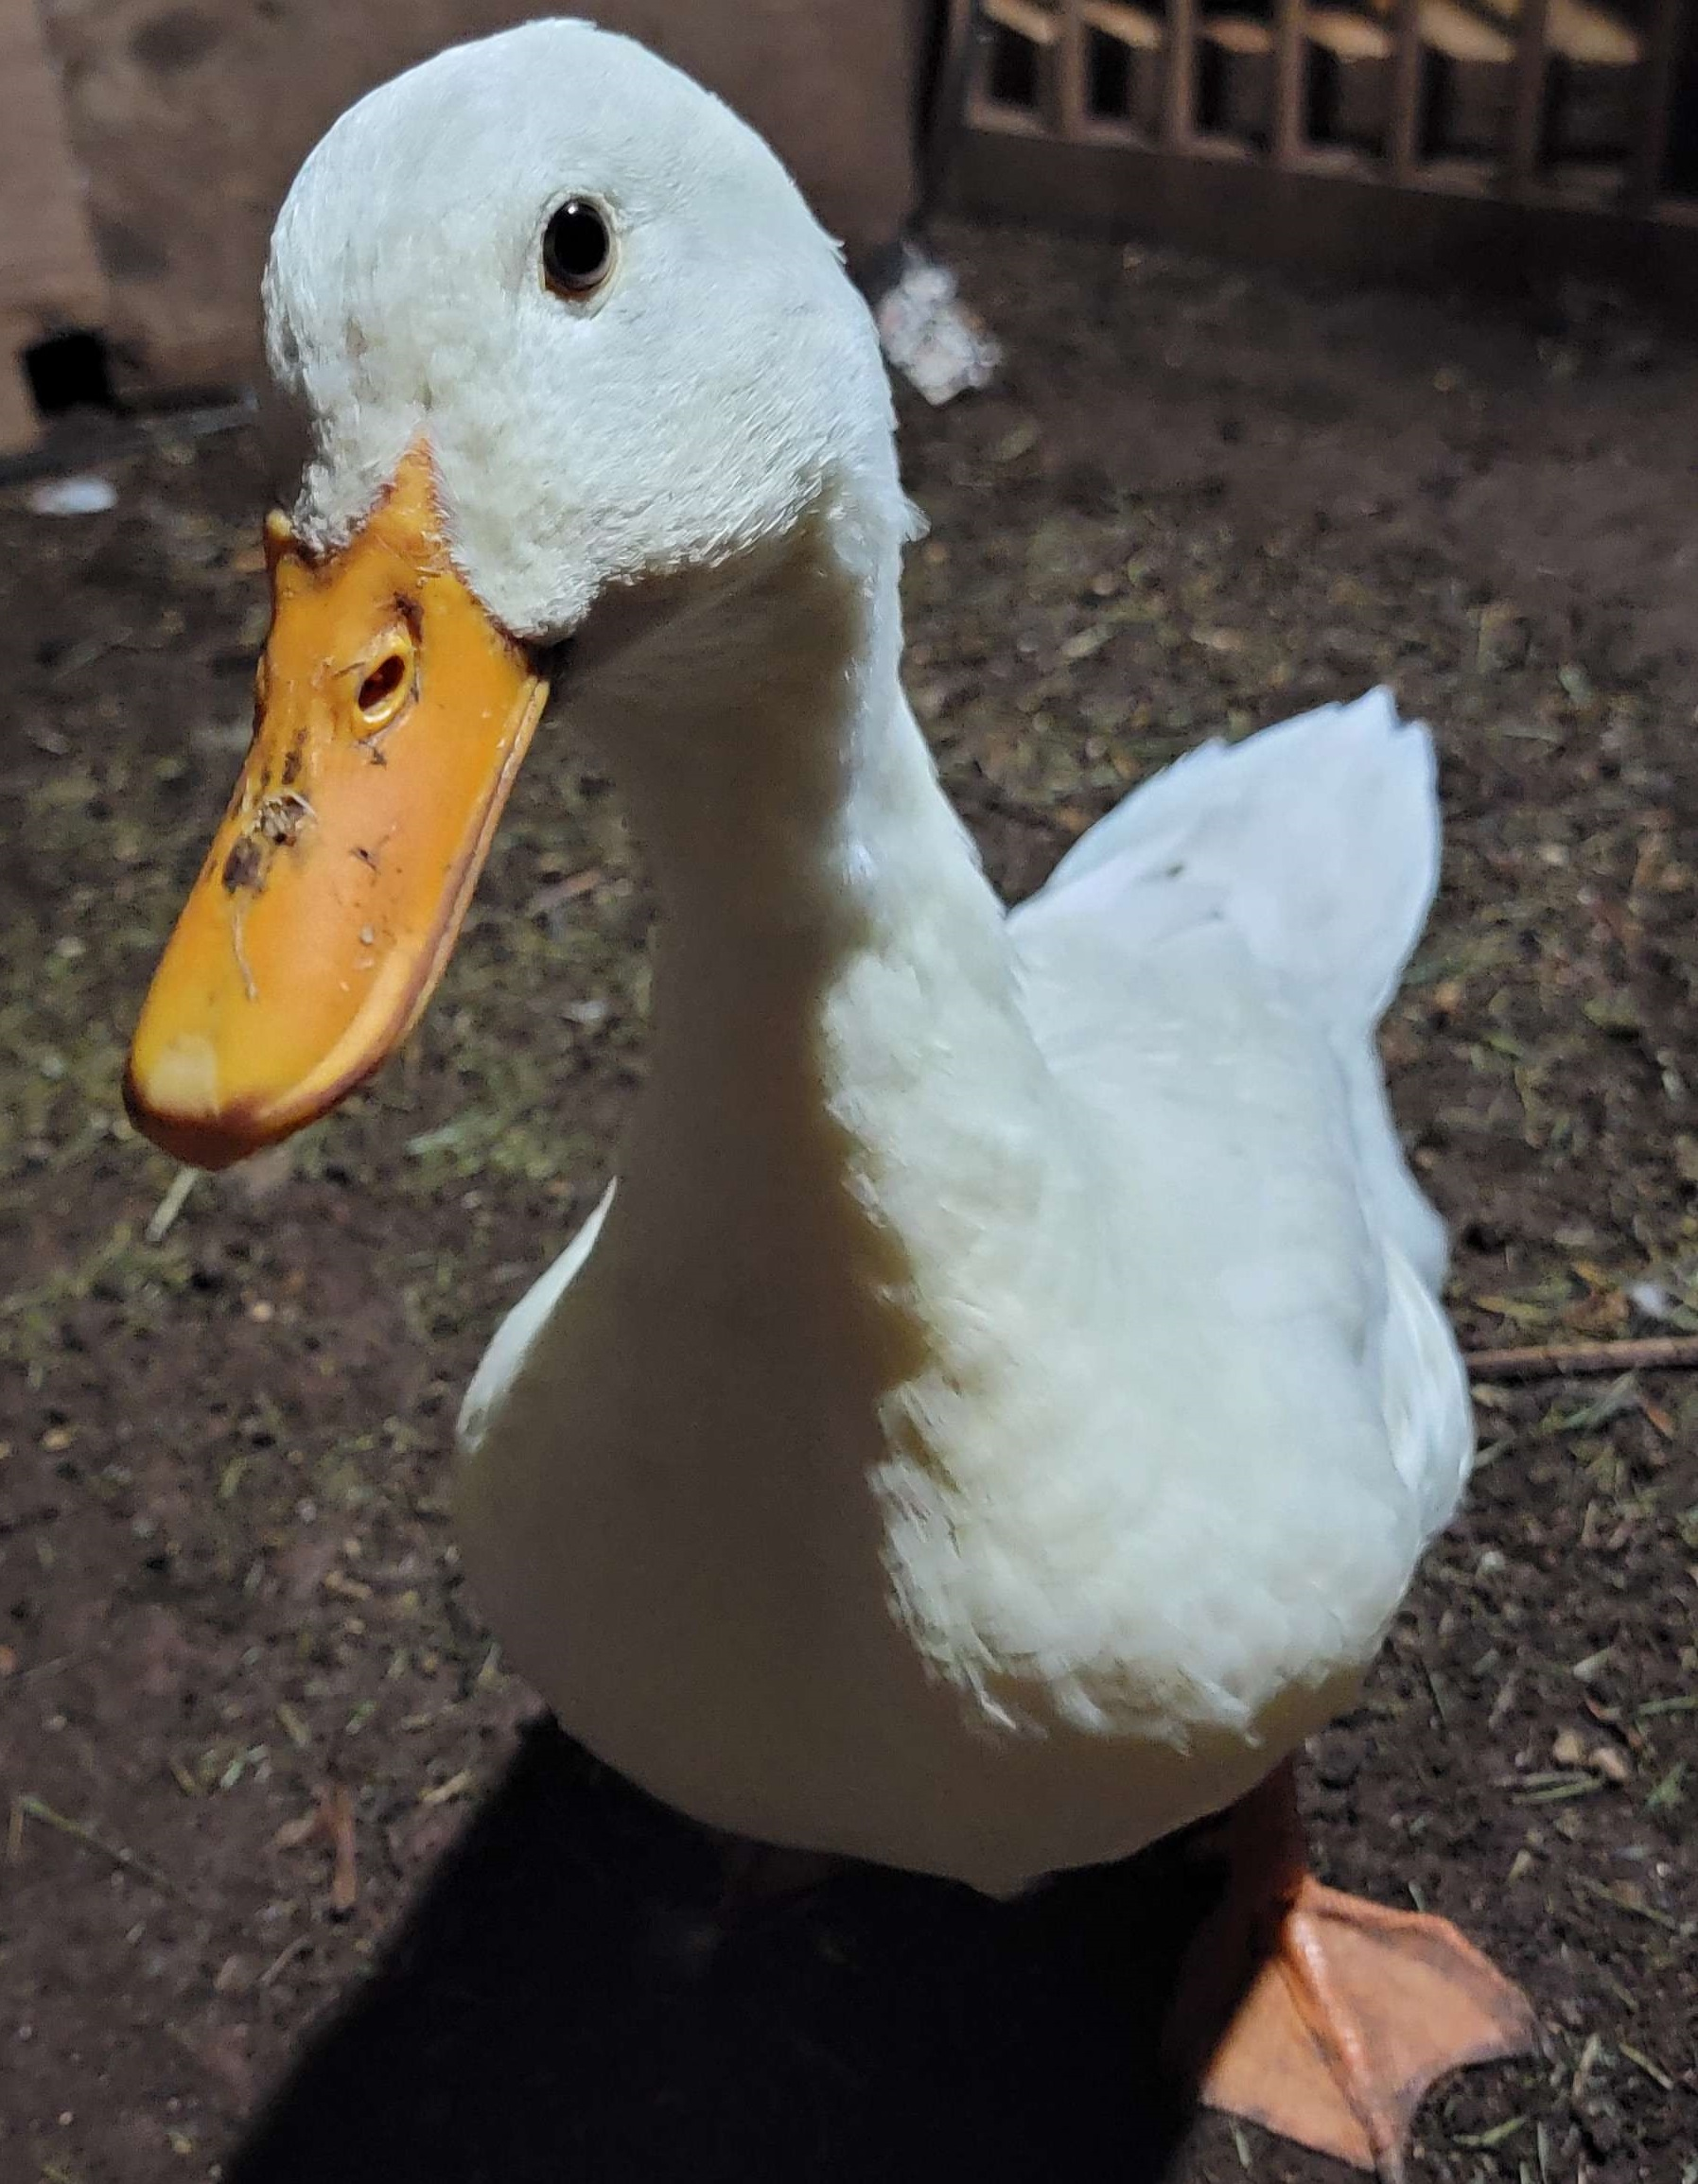
\includegraphics[width=0.15\linewidth]{New/20221011_213701.jpg}\footnote{Peep-a-Quack, your loyal Pekin duck.}
        \vfill
        \item Considering part (b), you no longer have lettuce in your burger. How much burger area will you consume?
        \vfill
        \item Upon further further inspection, this bread is not gluten free! You have celiac disease, so you relinquish the dreaded bread to Peep-a-Quack. For your dinner of tomato slices, how much tomato area are you eating?
        \vfill
        \vfill
    \end{enumerate}
\end{enumerate}



\end{document}
